\chapter{Background}
\label{chap:background}

In this chapter, we provide background knowledge that is commonly used across this dissertation.
Preliminaries specific to each chapter will be introduced later when they are needed.
Symbols used in this dissertation are summarized in~\cref{tbl:background-symbols}.

\begin{table}[t]
    \centering
    \caption{Summary of the symbols used in the dissertation}
    \label{tbl:background-symbols}
    \begin{tabular}{c|c}
        Symbol                      & Description                                                   \\
        \hline
        $\booldom$                  & The Boolean domain $\{\bot,\top\}$                            \\
        $x$                         & A Boolean variable                                            \\
        $l$                         & A literal (a variable or its negation)                        \\
        $\vl{l}$                    & The variable of $l$                                           \\
        $\as$                       & An assignment (a mapping from a variable set to $\booldom$)   \\
        $\as(x)$                    & The assigned value of $x$                                     \\
        $\av{V}$                    & The set of all assignments over variable set $V$              \\
        $\pf$                       & A quantifier-free formula                                     \\
        $\vf{\pf}$                  & The set of variables appearing in $\pf$                       \\
        $\as\models\pf$             & $\as$ satisfies $\pf$                                         \\
        $\pf_1\models\pf_2$         & Every satisfying assignment of $\pf_1$ also satisfies $\pf_2$ \\
        $\sat{\pf},\unsat{\pf}$     & $\pf$ is (un)satisfiable                                      \\
        $\model{\pf}$               & A satisfying assignment of $\pf$                              \\
        $\pcf{\pf}{x},\ncf{\pf}{x}$ & Positive and negative cofactors of $\pf$ w.r.t. $x$           \\
        $\pcf{\pf}{\as}$            & The resultant formula after cofactoring $\pf$ with $\as$      \\
        $C$                         & A clause (a disjunction of literals)                          \\
        $\Qf$                       & A quantified formula                                          \\
    \end{tabular}
\end{table}

\section{Propositional logic}
\label{sect:propositional-logic}

Boolean values \true and \false are represented by symbols $\top$ and $\bot$, respectively;
they are also treated as $1$ and $0$, respectively, in arithmetic computation.
Boolean connectives $\lnot, \lor, \land, \Rightarrow, \equiv$ are interpreted in their conventional semantics.
Given a set $V$ of variables,
an \textit{assignment} $\alpha$ is a mapping from each variable $x\in V$ to $\mathbb{B}=\{\top,\bot\}$,
and we denote the set of all assignments over $V$ by $\mathcal{A}(V)$.
An assignment $\alpha$ \textit{satisfies} a Boolean formula $\phi$ over a set $V$ of variables if $\phi$ yields $\top$ after substituting all occurrences of every variable $x\in V$ with its assigned value $\alpha(x)$ and simplifying $\phi$ under the semantics of Boolean connectives.
A Boolean formula $\phi$ over a set $V$ of variables is a \textit{tautology} if every assignment $\alpha\in \mathcal{A}(V)$ satisfies $\phi$.

We represent Boolean values \textsc{true} and \textsc{false} by symbols $\top$ and $\bot$, respectively.
In the sequel, a variable $x$ is assumed in the Boolean domain $\mathbb{B} = \{\top, \bot\}$.
A \emph{literal} is a variable (called a \emph{positive literal}) or the negation of a variable (called a \emph{negative literal}).
For a literal $l$, let $\mathtt{var}(l)$ denote the variable of $l$.
Boolean connectives $\neg, \vee, \wedge, \Rightarrow, \equiv$ are interpreted in their conventional meanings.

Let $\mathbb{B}=\{\top, \bot\}$, where $\top$ and $\bot$ denote logic \textsc{true} and \textsc{false}.
A \emph{literal} is a Boolean variable or its negation.
A \emph{clause} (resp. \emph{cube}) is a disjunction (resp. conjunction) of literals. A \emph{conjunctive normal form} (CNF) formula is a conjunction of clauses.
A Boolean formula $\phi$ over variables $X = \{x_1, \ldots, x_n\}$ induces a Boolean function mapping from $\mathbb{B}^n$ to $\mathbb{B}$.
The set of Boolean variables appearing in a Boolean formula $\phi$ is denoted as $\mathtt{vars}(\phi)$.
An \emph{assignment} $\tau$ on variables $X \subseteq \mathtt{vars}(\phi)$ of formula $\phi$ is a mapping from $X$ to $\mathbb{B}$.
An assignment $\tau$ is called a \emph{complete assignment} on $\mathtt{vars}(\phi)$ if $X=\mathtt{vars}(\phi)$; otherwise, it is called a \emph{partial assignment} on $\mathtt{vars}(\phi)$.
The formula of $\phi$ induced under the assignment $\tau$ on $X \subseteq \mathtt{vars}(\phi)$ is obtained by substituting every appearance of $x \in X$ in $\phi$ by $\tau(x)$, and is denoted as $\phi|_\tau$.
A complete assignment $\tau$ is called a \emph{satisfying} (resp. an \emph{unsatisfying}) \emph{(complete) assignment} for $\phi$ if $\phi|_\tau=\top$ (resp. $\phi|_\tau=\bot$).
Similarly, a partial assignment $\tau^+$ on $X \subset \mathtt{vars}(\phi)$ for $\phi$ is called a \emph{satisfying} (resp. an \emph{unsatisfying}) \emph{(partial) assignment} on $\mathtt{vars}(\phi)$ if for some (resp. every) assignment $\mu$ on $\mathtt{vars}(\phi)\setminus X$, $\phi$ valuates to $\top$ (resp. $\bot$) under the complete assignment obtained by combining $\tau$ and $\mu$.
In the sequel, we alternatively represent an assignment $\tau$ for $\phi$ as a cube.
A cube is called a \emph{minterm} when it corresponds to a complete assignment with respect to a specified set of variables.
A Boolean formula $\phi$ is called \emph{satisfiable} if there exists a satisfying complete assignment for $\phi$. We write $\mathtt{SAT}(\phi)=\top$ to denote $\phi$ is satisfiable.
A satisfying assignment of $\phi$ is also called a \emph{model} of $\phi$, denoted by $\phi.\mathrm{model}$.
On the other hand, if $\phi$ has no satisfying assignment, it is unsatisfiable and written as $\mathtt{SAT}(\phi)=\bot$.
%Therefore, a satisfying (resp. an unsatisfying) complete assignment for $\phi$ is also called a satisfying (resp. an unsatisfying) minterm of $\phi$, while a satisfying (resp. an unsatisfying) partial assignment is denoted as a satisfying (resp. an unsatisfying) cube, or a SAT (resp. an UNSAT) cube of $\phi$.

\subsection{Conjunctive normal form}
A \emph{clause} is a disjunction of literals.
A propositional Boolean formula $\phi$ is in \emph{Conjunctive Normal Form} (CNF) if $\phi$ is a conjunction of clauses.
A variable $x$ is said to be \emph{pure} in a formula if its appearances in the formula are all in the \emph{positive phase} $x$ or in the \emph{negative phase} $\neg x$.
A \emph{cube} is a conjunction of literals.
In the sequel, we assume propositional Boolean formulas are in CNF.

\subsection{Satisfiability}
A Boolean formula $\phi$ over a set of variables $X=\{x_1, \ldots, x_n\}$ defines a unique Boolean function $\mathbb{B}^n \rightarrow \mathbb{B}$.
Let $\mathtt{vars}(\phi)$ denote the set of variables appearing in a Boolean formula $\phi$.
An \emph{assignment} $\tau$ over a set of variables $X \subseteq \mathtt{vars}(\phi)$ for a formula $\phi$ is a mapping $\tau: X \rightarrow \mathbb{B}$.
An assignment $\tau: X \rightarrow \mathbb{B}$ is a \emph{complete assignment} for formula $\phi$ if $X=\mathtt{vars}(\phi)$; otherwise, i.e., $X \subset \mathtt{vars}(\phi)$, it is a \emph{partial assignment}.
Given a Boolean formula $\phi$ and an assignment $\tau$ over $\mathtt{vars}(\phi)$, the \emph{cofactor} of $\phi$ under $\tau$, denoted by $\phi|_{\tau}$, is derived by substituting every occurrence of each variable $x \in \mathtt{vars}(\phi)$ in $\phi$ by $\tau(x)$.
If $\phi|_{\tau}=\top$, we call $\tau$ a satisfying assignment of $\phi$.
The satisfiability problem of a Boolean formula $\phi$ asks whether or not $\phi$ has a satisfying assignment.
We write $\mathtt{SAT}(\phi)=\top$ to denote that $\phi$ is satisfiable.
A satisfying assignment of $\phi$ is also called a \emph{model} of $\phi$.
%denoted by $\phi.\mathrm{model}$.
On the other hand, if $\phi$ has no satisfying assignment, it is unsatisfiable and written as $\mathtt{SAT}(\phi)=\bot$.
Given two Boolean formulas $\phi$ and $\psi$, we write $\phi \models \psi$ if every satisfying assignment for $\phi$ also satisfies $\psi$.
In the sequel, we alternatively represent an assignment $\tau$ as a cube, a clause $C$ as a set of literals, and a CNF formula as a set of clauses.

\subsection{Minterm generalization}
Consider a CNF formula $\phi(X,Y)$, where $X$ and $Y$ are two disjoint sets of Boolean variables.
Given an assignment $\tau$ on $X$, if $\phi(X,Y)|_\tau$ is satisfiable (resp. unsatisfiable), $\tau$ is called a SAT (resp. an UNSAT) minterm of $\phi$ on $X$.
The generalization process of a SAT or an UNSAT minterm $\tau$ aims at expanding it to a cube $\tau^+$, while maintaining the satisfiability of $\phi(X,Y)|_{\tau^+}$ the same as $\phi(X,Y)|_\tau$.
\begin{example}\label{ex:assign}
    Consider formula $\phi(x_1, x_2, y_1, y_2)=x_1 \wedge (\neg x_2 \vee y_1 \vee y_2)$. The assignment $\tau = x_1 x_2$ on $X$, i.e., $\tau(x_1)=\top, \tau(x_2)=\top$, is a satisfying assignment, or a SAT minterm, of $\phi$ on $X$ as $\phi|_\tau$ is satisfiable by assignment $\mu = y_1y_2$.
    On the other hand, the partial assignment $\tau^+ = \neg x_1$, i.e., $\tau^+(x_1)=\bot$, is an unsatisfying partial assignment, or an UNSAT cube, of $\phi$ as $\phi|_{\tau^+}$ is unsatisfiable.
\end{example}

\subsubsection{Minimum Satisfying Assignment}
For a CNF formula $\phi(X,Y)$, let $\tau$ be a SAT minterm on $X$ and let $\mu$ be a satisfying assignment for $\phi(X,Y)|_\tau$ on $Y$. To generalize $\tau$ into a cube, one can find a subset of literals from $\tau$ and $\mu$ that are able to satisfy all clauses in $\phi$ while the number of literals taken from $\tau$ is as few as possible. If some literals in $\tau$ are irrelevant to the satisfiability, they can be dropped from $\tau$, thus expanding $\tau$ to a SAT cube $\tau^+$. If in the SAT cube $\tau^+$, the number of literals taking from $\tau$ is minimized, $\tau^+$ is called the \textit{minimum satisfying assignment}. The process of finding the minimum satisfying assignment is also known as finding the \textit{minimum hitting set}.

\subsubsection{Minimum Conflicting Assignment}
Given an UNSAT minterm $\tau$ of a CNF formula $\phi$,
modern SAT solvers, such as \minisat~\cite{Een2003Solver,Een2003Incremental},
are able to analyze the reason of unsatisfiability,
which is represented as a conjunction of literals in $\tau$ causing the conflict.
If some literals in $\tau$ are irrelevant to the conflict, they are dropped from $\tau$, thus expanding $\tau$ to an UNSAT cube $\tau^+$.
If the number of literals in the UNSAT cube $\tau^+$ is minimized, $\tau^+$ is called the \textit{minimum conflicting assignment}.
The process of finding the minimum conflicting assignment is also known as finding the \textit{minimum UNSAT core}.


\subsection{Binary decision diagram}
\begin{frame}
    \frametitle{Background}
    \begin{block}{Stochastic Boolean Satisfiability (SSAT)}
        $\Qf=Q_1 x_1,\ldots,Q_n x_n.\pf$
        \pause
        \begin{itemize}
            \item $Q_1 x_1,\ldots,Q_n x_n$: quantification structure, $Q_i \in \{\random{p},\exists\}$ (\emph{prefix})
                  \pause
            \item $\pf$: quantifier-free formula over $\{x_1,\ldots,x_n\}$ (\emph{matrix})
        \end{itemize}
    \end{block}
    \pause
    \begin{block}{Computational Rules for Satisfying Probability}
        Let $x$ be the outermost variable in the prefix:
        \pause
        \begin{enumerate}
            \item[a)] $\spb{\top}=1$,
                  \pause
            \item[b)] $\spb{\bot}=0$,
                  \pause
            \item[c)] $\spb{\Qf}=\max\{\spb{\ncf{\Qf}{x}},\spb{\pcf{\Qf}{x}}\}$, if $x$ is quantified by $\exists$,
                  \pause
            \item[d)] $\spb{\Qf}=(1-p)\spb{\ncf{\Qf}{x}}+p\spb{\pcf{\Qf}{x}}$, if $x$ is quantified by $\random{p}$.
        \end{enumerate}
    \end{block}
\end{frame}

\begin{frame}
    \frametitle{Background}
    \begin{block}{Example: Computation of Satisfying Probability}
        \abovedisplayskip=0pt
        \begin{align*}
             & \Qf=\random{0.5} x_1, \exists y_1, \random{0.5} x_2, \exists y_2. \pf \\
             & \pf=(x_1 \lor \lnot y_1)
            (\lnot x_1 \lor y_1)
            (\lnot x_1 \lor \lnot x_2 \lor y_2)
            (x_1 \lor \lnot y_2)
            (x_2 \lor \lnot y_2)
        \end{align*}
    \end{block}\pause
    \begin{figure}
        \centering
        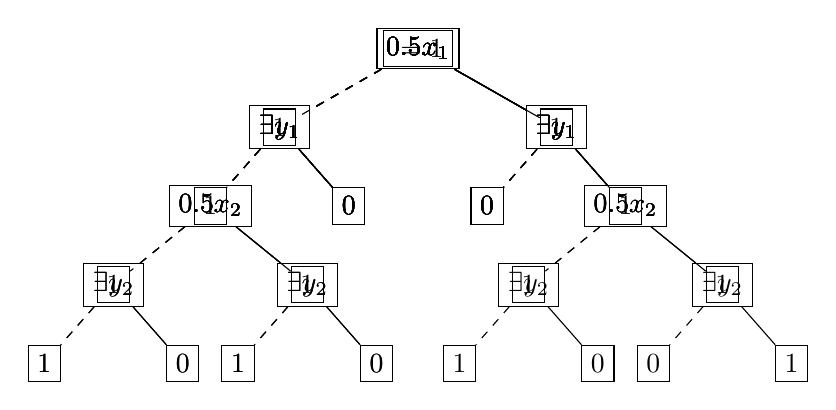
\begin{tikzpicture}[
                baseline,
                level distance=10mm,
                level 1/.style={sibling distance=10em},
                level 2/.style={sibling distance=5em},
                level 3/.style={sibling distance=7em},
                level 4/.style={sibling distance=5em},
                every node/.style={solid,draw},
                positive/.style={edge from parent/.style={solid,draw}},
                negative/.style={edge from parent/.style={dashed,draw}}]

            \action<2>{\node{$\random{0.5} x_1$};}
            \action<3>{\node{$\random{0.5} x_1$}
                child[negative]{node{$\exists y_1$}}
                child[positive]{node{$\exists y_1$}};}
            \action<4>{\node{$\random{0.5} x_1$}
                child[negative]{node{$\exists y_1$}
                        child[negative]{node{$\random{0.5} x_2$}}
                        child[positive]{node{$0$}}}
                child[positive]{node{$\exists y_1$}};}
            \action<5>{\node{$\random{0.5} x_1$}
                child[negative]{node{$\exists y_1$}
                        child[negative]{node{$\random{0.5} x_2$}}
                        child[positive]{node{$0$}}}
                child[positive]{node{$\exists y_1$}
                        child[negative]{node{$0$}}
                        child[positive]{node{$\random{0.5} x_2$}}};}
            \action<6>{\node{$\random{0.5} x_1$}
                child[negative]{node{$\exists y_1$}
                        child[negative]{node{$\random{0.5} x_2$}
                                child[negative]{node{$\exists y_2$}
                                        child[negative]{node{$1$}}
                                        child[positive]{node{$0$}}}
                                child[positive]{node{$\exists y_2$}
                                        child[negative]{node{$1$}}
                                        child[positive]{node{$0$}}}}
                        child[positive]{node{$0$}}}
                child[positive]{node{$\exists y_1$}
                        child[negative]{node{$0$}}
                        child[positive]{node{$\random{0.5} x_2$}}};}
            \action<7>{\node{$\random{0.5} x_1$}
                child[negative]{node{$\exists y_1$}
                        child[negative]{node{$\random{0.5} x_2$}
                                child[negative]{node{$\exists y_2$}
                                        child[negative]{node{$1$}}
                                        child[positive]{node{$0$}}}
                                child[positive]{node{$\exists y_2$}
                                        child[negative]{node{$1$}}
                                        child[positive]{node{$0$}}}}
                        child[positive]{node{$0$}}}
                child[positive]{node{$\exists y_1$}
                        child[negative]{node{$0$}}
                        child[positive]{node{$\random{0.5} x_2$}
                                child[negative]{node{$\exists y_2$}
                                        child[negative]{node{$1$}}
                                        child[positive]{node{$0$}}}
                                child[positive]{node{$\exists y_2$}
                                        child[negative]{node{$0$}}
                                        child[positive]{node{$1$}}}}};}
            \action<8>{\node{$\random{0.5} x_1$}
                child[negative]{node{$\exists y_1$}
                        child[negative]{node{$\random{0.5} x_2$}
                                child[negative]{node{$1$}}
                                child[positive]{node{$1$}}}
                        child[positive]{node{$0$}}}
                child[positive]{node{$\exists y_1$}
                        child[negative]{node{$0$}}
                        child[positive]{node{$\random{0.5} x_2$}
                                child[negative]{node{$1$}}
                                child[positive]{node{$1$}}}};}
            \action<9>{\node{$\random{0.5} x_1$}
                child[negative]{node{$\exists y_1$}
                        child[negative]{node{$1$}}
                        child[positive]{node{$0$}}}
                child[positive]{node{$\exists y_1$}
                        child[negative]{node{$0$}}
                        child[positive]{node{$1$}}};}
            \action<10>{\node{$\random{0.5} x_1$}
                child[negative]{node{$1$}}
                child[positive]{node{$1$}};}
            \action<11>{\node{$\spb{\Qf}=1$};}
        \end{tikzpicture}
    \end{figure}
\end{frame}

\begin{frame}
    \frametitle{Express Model-Counting Variants with SSAT}
    \begin{table}[t]
        \centering
        \begin{tabular}{c|c}
            Variant            & SSAT encoding                                                               \\
            \hline
            Unweighted         & $\random{0.5}x_1,\ldots,\random{0.5}x_n.\pf$                                \\
            Weighted           & $\random{p_1}x_1,\ldots,\random{p_n}x_n.\pf$                                \\
            Projected          & $\random{0.5}x_1,\ldots,\random{0.5}x_n,\exists y_1,\ldots,\exists y_m.\pf$ \\
            Maximum            & $\exists x_1,\ldots,\exists x_n,\random{0.5}y_1,\ldots,\random{0.5}y_m.\pf$ \\
            Weighted projected & $\random{p_1}x_1,\ldots,\random{p_n}x_n,\exists y_1,\ldots,\exists y_m.\pf$ \\
            Weighted maximum   & $\exists x_1,\ldots,\exists x_n,\random{p_1}y_1,\ldots,\random{p_m}y_m.\pf$ \\
        \end{tabular}
    \end{table}
\end{frame}

\begin{frame}
    \frametitle{Background}
    \begin{block}{Game-Theoretical Interpretation of SSAT}
        $\Qf=Q_1 x_1,\ldots,Q_n x_n.\pf$, $Q_i \in \{\random{p},\exists\}$
        \pause
        \begin{itemize}
            \item $\random{p}$: nondeterministic factors
                  \pause
            \item $\exists$: an agent who plays under uncertainty
                  \pause
            \item $\pf$: game matrix
                  \pause
            \item $\spb{\Qf}$: the maximum winning probability of the agent
                  \pause
            \item \alert{Skolem functions}: a winning/optimization strategy of the agent
        \end{itemize}
    \end{block}\pause
    \begin{block}{Example: Skolem Functions}
        \abovedisplayskip=0pt
        \belowdisplayskip=0pt
        \begin{align*}
             & \Qf=\random{0.5} x_1, \exists y_1, \random{0.5} x_2, \exists y_2. \pf \\
             & \pf=(x_1 \lor \lnot y_1)
            (\lnot x_1 \lor y_1)
            (\lnot x_1 \lor \lnot x_2 \lor y_2)
            (x_1 \lor \lnot y_2)
            (x_2 \lor \lnot y_2)
        \end{align*}
        \pause
        \begin{itemize}
            \item Variable $y_1$: $f_1(x_1)=x_1$; variable $y_2$: $f_2(x_1,x_2)=x_1 \land x_2$
        \end{itemize}
    \end{block}
\end{frame}
\section{Model counting}
\label{sect:related-work-model-counting}